% !TEX root =  ../supplementary.tex
\section{Web Application for Practical Use of Personalized Schedule of Biopsies}

We implemented our methodology in a web-application to assist patients and doctors in better decision making. It works on desktop as well as mobile devices. It is hosted at \url{https://emcbiostatistics.shinyapps.io/prias_biopsy_recommender/}. 

\begin{figure}[!htb]
\centerline{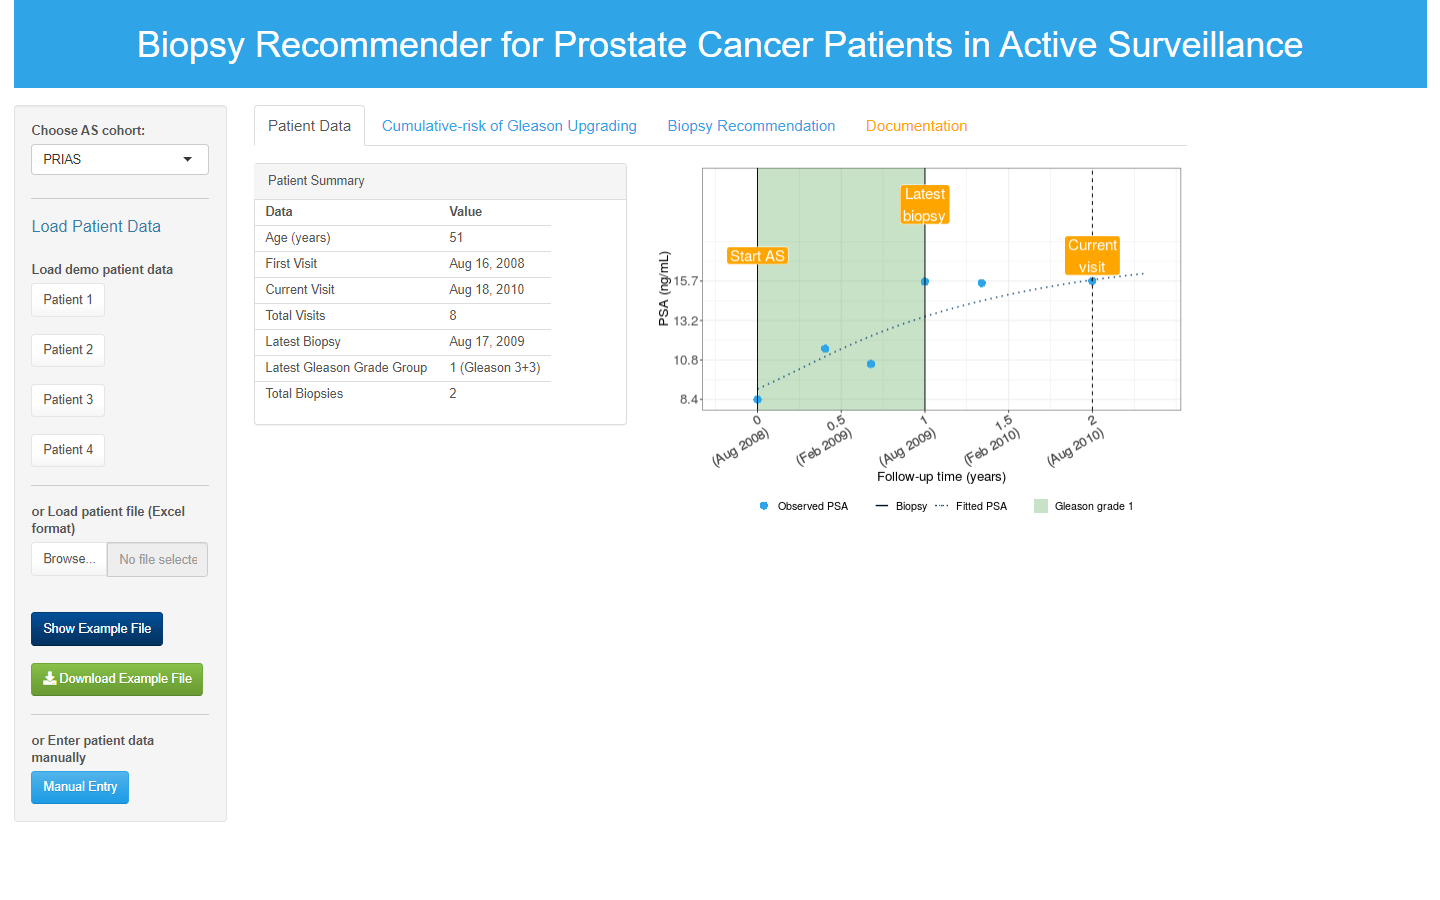
\includegraphics[width=\columnwidth]{images/app/landing_page.png}}
\caption{Landing page of the web-application. Panel on the left allows users to load patient data and panel on the right provides information. Patient data can be entered manually, or via Excel files. In addition, demo patient data is already uploaded to assist users in understanding the web-application.}
\label{fig:landing_page}
\end{figure}

\begin{figure}
\centerline{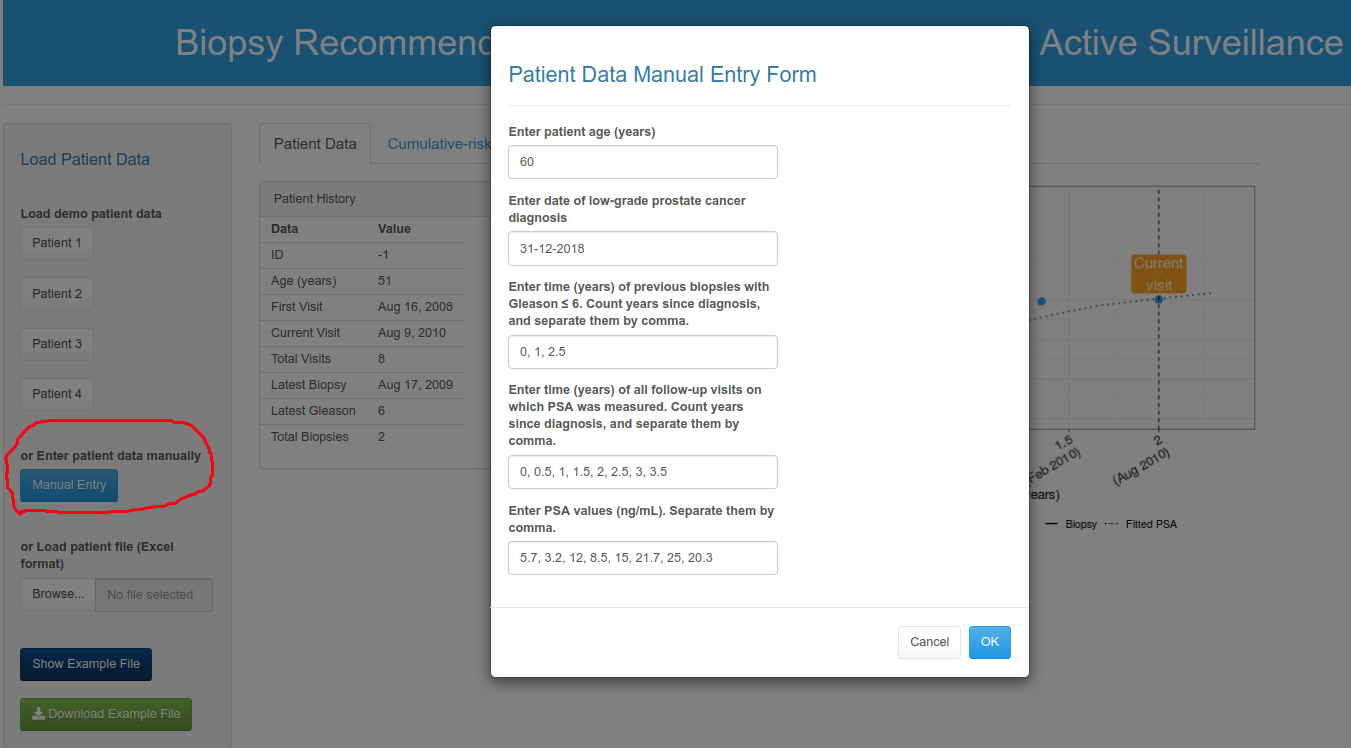
\includegraphics[width=\columnwidth]{images/app/manual_entry.png}}
\caption{Patient data can be entered manually.}
\label{fig:manual_entry}
\end{figure}

\begin{figure}
\centerline{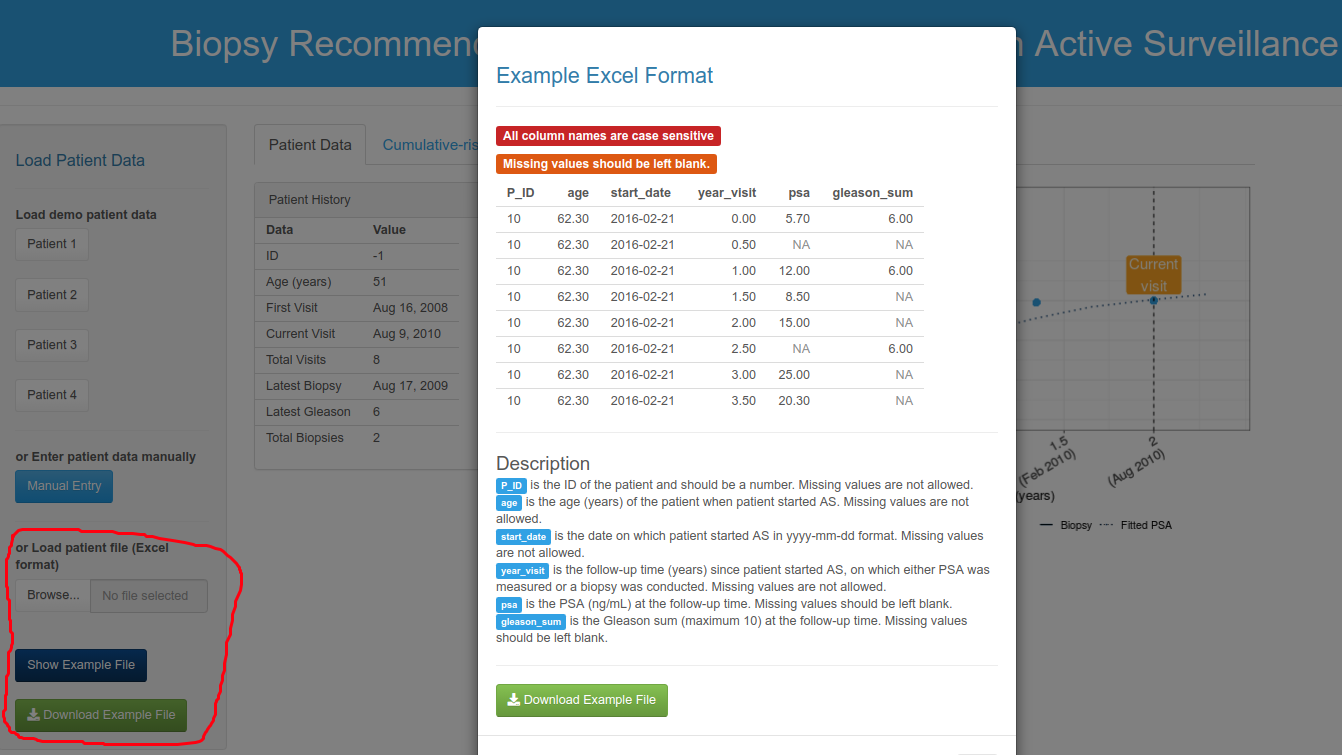
\includegraphics[width=\columnwidth]{images/app/excel_entry.png}}
\caption{Patient data can be uploaded via Excel sheets. Example Excel sheet format is provided within the web-application. In addition, users can download an Excel template to fill patient data.}
\label{fig:excel_entry}
\end{figure}

\begin{figure}
\centerline{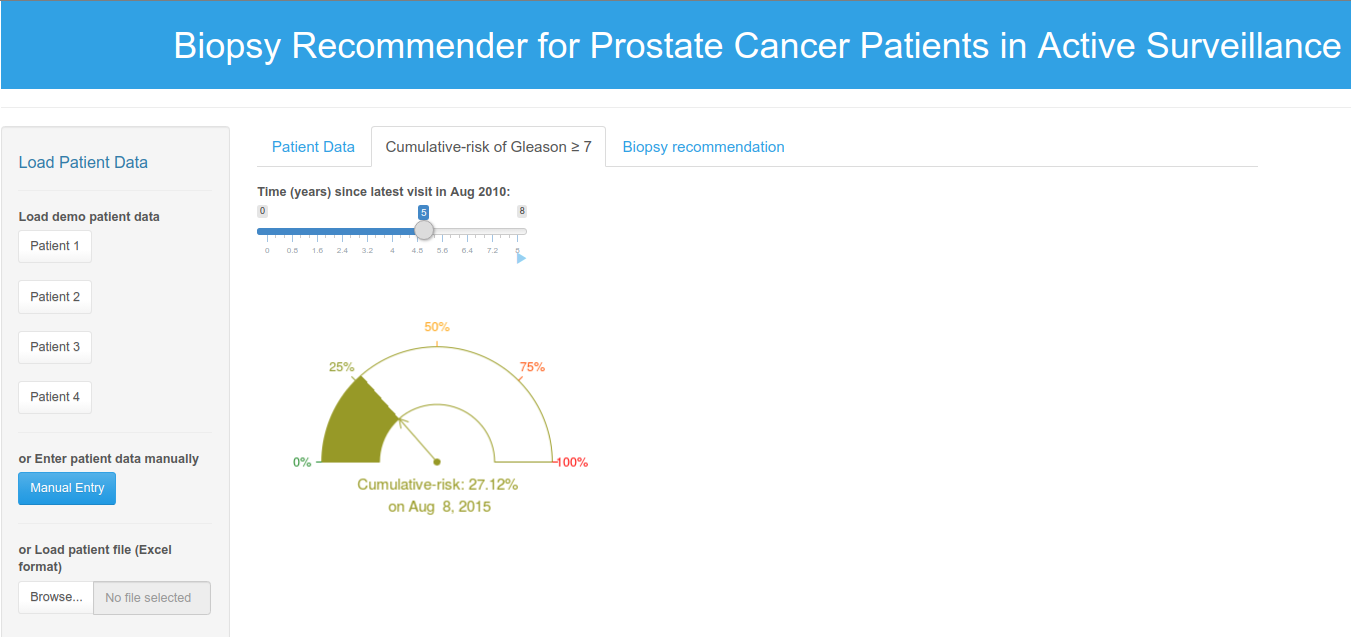
\includegraphics[width=\columnwidth]{images/app/cum_risk.png}}
\caption{Second tab panel provides patient's personalized cumulative-risk of Gleason $\geq$ 7 since his latest biopsy.}
\label{fig:cum_risk}
\end{figure}

\begin{figure}
\centerline{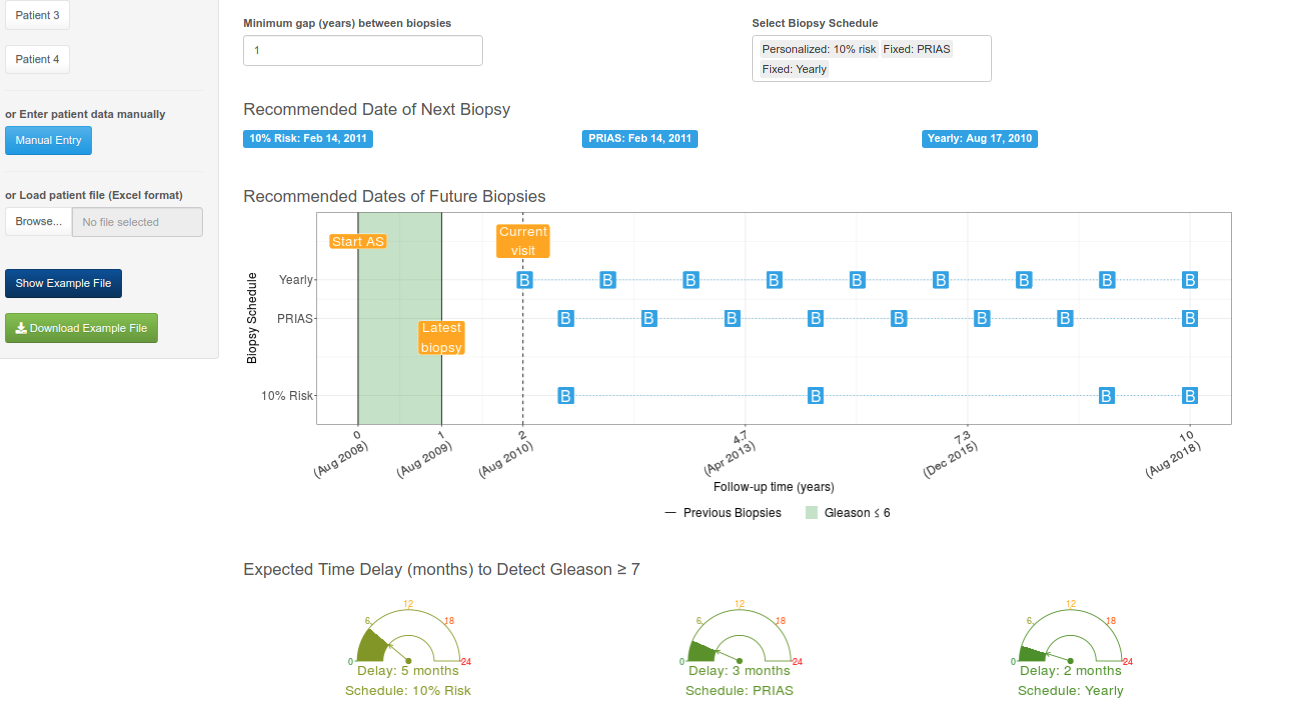
\includegraphics[width=\columnwidth]{images/app/biopsy_recommendation.png}}
\caption{Third tab panel provides personalized and fixed biopsy schedule options as well as the expected time delay in detection of Gleason $\geq$ 7 for each of the schedules.}
\label{fig:biopsy_recommendation}
\end{figure}
